\chapter{Materials and Methods}

\section{Wireless Sensor Networks}
A Wireless Sensor Network (WSN) is a collection of small, low-cost, low-power sensor nodes that do not only have sensing capacities but also computing capacities. Additionally, these nodes are able to communicate with each other via a wireless medium. Such a WSN deployed in an area of interest makes it possible to monitor the area in a desired way enabling applications for environmental and habitat monitoring, analysis of structures, or localization and tracking.

The typical architecture of a WSN includes one node that functions as the sink. This means that this node is the connection to a PC or the Internet to bring the information collected by the nodes to the user. All the nodes then are spread over the area of interest. When placing the nodes it is important that each node can somehow communicate with the sink, may it be a direct connection or an indirect over other nodes. Are all the nodes in direct range of each other it is a single-hop network meaning each node can transmit a message directly to all the other nodes. Otherwise the network is called multi-hop. This means nodes can not necessarily transmit messages directly to all the other nodes but may need to transmit the message over other nodes that forward it to the destination.

The application running on the node is designed specifically for the purpose of the WSN. Since the nodes should operate independently, they are often powered by battery. This makes power one of the constrains of a WSN and applications need to be designed to have a low power consumption. Moreover the application designed for the nodes needs to take the constrains of low computation capability and low storage of the sensor nodes into account. \cite{Wsn} \cite{Tinyos} 

%-Able to communicate with each other. 
%-Placed to monitore an area of intrest.
%-Charasteristics.
%	-Dense node Deployment
%	-Battery Powered
%	- Application Specific
%	-Many to one Traffc patter
%-Constrains.	
%	-Energy
%	-computation
%	-storage
%	-unreliable sensor nodes
	
%-Typical WSN architekture (Pc sink nodes )
%-Multi hop network not multi hop networks
%-Stuff to take care of because of constrains

%TinyOS: An Operating System for Sensor Networks:
%-Consists of potentialy thousands of nodes
%-small, flexible, lowcost nodes that interact with their environment
%-applications ranging from environmental and habitat monitoring [11, 51], seismic analysis of structures [10], and object localization and tracking [68].


\section{Radio Tomographic Imaging}
Radio Tomographic Imaging (RTI) is a method to localize people inside an area covered by a WSN. To do so, the WSN monitors the received signal strength (RSS) of each link inside the network by letting each node send broadcast messages over radio. Whenever a person stays or moves inside the monitored area, it affects the RSS of some or all links. The changes can then be processed and a position of the person can be estimated. This makes it possible to localize a person without it having to carry any device.  \cite{RtiMulti}
\section{Multi-Spin}
When monitoring the RSS of each link inside a WSN, it is important to take into account that not only changes inside the environment can affect the RSS. Also multiple messages sent at the same time interfere with each other and distort the measured change of the RSS. To counteract this, a method to schedule the messages in a way that only one node sends at a given point in time is needed. In the literature the Multi-Spin \cite{RtiMulti} algorithm is suggested that defines for each node a point in time when it should send its message.

In Multi-Spin, time is divided into $slots$ and $cycles$ where a $cycle$ is the time all the nodes need to send one message each. Then a $cycle$ is divided by the number of nodes inside the network resulting in one $slot$ for each node, as shown in Figure \ref{fig:multi}. Now each node sends in one of these slots. The order in which the nodes send is defined by their ID. To make this possible, the nodes need to somehow synchronize at the beginning. Therefore each node broadcasts messages until one message is received by the nodes. Then the nodes synchronize their time with that message, define their timeslots and start sending in the order of their IDs. Whenever a node receives a message, it can calculate the time until the next $cycle$, so the nodes stay synchronized all the time. \cite{RtiMulti}

\begin{figure}[htbp]
	\centering
    \includegraphics[scale=0.8]{content/images/Multispin}
   	\caption{Time is devided into $slots$ and $cycles$. A $cycle$ is the time all the nodes need to send their message. A $cycle$ is then divided by the number of nodes to create a $slot$ for each node where it can send its message. \cite{RtiMulti}}
    \label{fig:multi}
\end{figure}

For the collection of the RSS measurements an extra node that overhears all the messages is connected to a PC. The nodes include their ID and the last RSS measurements inside their messages. The extra node now receives the messages from all the other nodes and forwards them to the PC.  \cite{RtiMulti}

This method is fast, efficient and stable. However it only works under the assumption that all the nodes can hear each other. When not all the nodes hear each other, the synchronization would not be that accurate, making it necessary to resynchronize for each $cycle$. Moreover the data collection does not work at all. There is no node that is able to hear all the other nodes and therefore collect the information by simply listening to the sent messages.
Therefore a different method is needed for a widely spread multi-hop network.

%should be explained in more detail
%very short time because highly optimized without a real time os benethe it
%not possible inside a multi hop enviroment
%every round needs a time sinchronization
%data collection not possible like that
%very cool but not sufficient in a multi hop enviroment
\section{Collection Tree Protocol}
To collect data from a multi-hop WSN, multiple data collection protocols exist. One of these is the Collection Tree Protocol (CTP). The CTP creates paths in form of trees. The nodes can then send their data along this path to a collection point. To schedule the forwarding of messages, each node implements a message queue. 

To create the paths, every node maintains the cost of its path to the collection point. The cost of a node's path is the cost of the link between itself and its parent added to the cost of its parent's path. Collection points have a path cost of zero. Now all the nodes send broadcast messages in a specific pattern which include the node's path costs. If a node receives a broadcast message that provides a smaller path cost, it can adjust its path to the new one.

Whenever a node now needs to send data, it can simply send it to its parent which will put the message inside its message queue and then forward it whenever it is possible. This makes it a good collection protocol for continuous data collection since nodes can send data whenever they have some, it recalibrates itself continuously and has high packet delivery rate. \cite{CTP}

The problem with collecting the signal strength information for RTI is that it needs to be done at a specific point in time to not distort the measurements. This means a method is needed to start the collection and to know when it is finished. 
\section{Wireles Sonsor Network Testbed}
\label{chp:mat_testbed}
A Wireless Sensor Network testbed is a WSN deployed in a controlled environment to test applications. This creates a realistic test environment showing not only the theoretical functionality like a simulation but also makes it possible to examine communication loss, energy constraints and the influence of the real environment.  

On the third floor of the SA building at the University of Duisburg-Essen such a WSN testbed is located. It is set up as a tool for researches on WSNs in an indoor environment. It covers half of the building including a large main corridor, two laboratories, two smaller corridors leading to three offices each, seven smaller storage rooms, an elevator and one server room. The arrangement of the rooms is laid out in Figure \ref{fig:testbed}. All in all, the area covers $531\ m^2$. All the rooms are in daily use by the people working in the offices and the laboratories, keeping the area under constant change.

\begin{figure}[htbp]
	\centering
    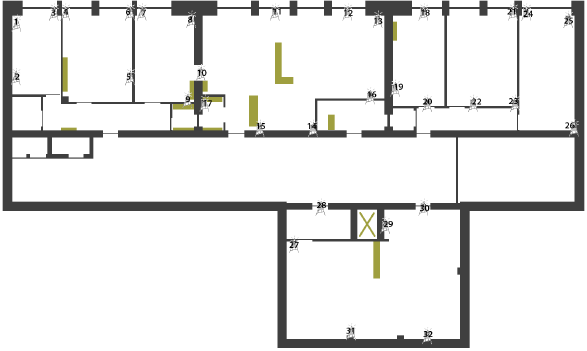
\includegraphics[scale=0.75]{content/images/Testbed}
   	\caption{Floor plan of the area where the testbed is located. The position of the nodes is shown by the numbered antennas.}
    \label{fig:testbed}
\end{figure}

To monitor the area, 32 nodes are distributed over the rooms like shown in Figure \ref{fig:testbed}. The nodes are only placed inside the offices and laboratories and are not always placed at the same height. To make programming of the devices easy, all the devices are connected to Raspberry Pis via USB. A script then makes it possible to copy the source code to all the Raspberry Pis where the code is compiled and then sent to each node individually. The connection to the Raspberry Pis makes it also possible to collect information directly from each node individually over serial forwarders running on the Raspberry Pis.

\subsection{TelosB Mote}
\label{chp:TelosB}
The sensor nodes used for the Testbed are Crossbow's TelosB Motes. The Crossbow TelosB Mote is an open source platform for researchers developed by the University of California, Berkeley. It provides an 8 MHz Texas Instrument MSP430 low power microcontroller with 10kB RAM that is programmable via a USB connector. For communication it includes an IEEE 802.15.4 compliant radio frequency transceiver with an embedded antenna. This makes transmissions in a frequency band from 2.4 to 2.4835 GHz possible. Moreover the Crossbow TelosB Mote has a light sensor, an infra-red sensor, a humidity sensor and a temperature sensor installed making it possible to monitor the environment. Last, it has three LED lights installed that can be used for visual output of the mote. The USB connector that can be used to program the microcontroller can also be used to exchange data with and to power the Crossbow TelosB Mote. If it is not connected via USB it can also be powered by two AA batteries. \cite{Telosb}

\begin{figure}[htbp]
	\centering
    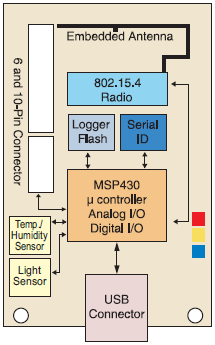
\includegraphics[scale=0.7]{content/images/Mote1}
   	\caption{The structure of the Crossbow TelosB Mote and the included components. \cite{Telosb}}
    \label{fig:telosb}
\end{figure}
 
\subsection{TinyOS}
TinyOS is an operating system for embedded systems, designed to manage the limited resources and power, and to provide reactive concurrency and flexibility. It is widely used by multiple research groups and companies worldwide to support their applications.

The main task of TinyOS is to schedule tasks and events to provide safe concurrent operations. Additionally it also provides a large amount of reusable system components, like timers, sender or receiver, that provide a huge variety of functionalities. When compiling an application, only the TinyOS components that are used by the application are included creating an application-specific OS.

To provide functionality, each component can have three different types of computational abstractions. First there are commands making it possible for other components to call a functionality of the component providing the command. Then there are events which can be signaled by a component. A component receiving the event can then react to it and act accordingly. These two constructs make interaction between components possible. Last, for internal functionality of components there are tasks. These can be posted by a component and then are executed when it is their turn. 

Whenever a command, event or task gets called it is pushed into the queue of the TinyOS scheduler. The scheduler then executes the tasks inside the queue using a FIFO scheduling policy. \cite{Tinyos}     

\subsubsection{Programming for TinyOS}
Applications for TinyOS are written in nesC which is a C dialect and integrates the possibility to implement configurations, modules, interfaces, commands, events and tasks. An application consists of components, represented by a nesC module, that provide and use interfaces. The components implement the functionality of the application. All the commands and events a component provides are defined by an interface. Moreover an application for TinyOS also has a configuration that defines which components are used and describes their connections.   

The Listings \ref{lis:Components}, \ref{lis:interface} and \ref{lis:configuration} show an example application for TinyOS with two components of which one provides an interface and the configuration for the application. This example shows the connections between components, interfaces and the configuration and also shows the use of commands, events and tasks. In Listing \ref{lis:Components} the two components $MainComponent$ and $ExampleC$ are represented. $MainComponent$ uses two interfaces. The first one is the $Boot$ interface. It requires the component to implement the $Boot.booted()$ event. This event is the first event signaled by TinyOS after the node booted. Moreover the $MainComponent$ uses the $ExampleI$ interface that is defined in Listing \ref{lis:interface}. It requires the component to implement the $exampleDone(error\_t\ error)$ event. The $ExampleI$ interface is provided by the $ExampleC$ component and requires it to implement the $startExample()$ command. Moreover the $ExampleC$ component implements a task $doSomething()$.

Now to connect everything, the configuration $Application$ in Listing \ref{lis:configuration} first defines all the components needed for the application. The first component used in this application is the $MainC$ component that provides the $Boot$ interface and is given by TinyOS. Next, there are the two components from Listing \ref{lis:Components}. Now the configuration needs to connect the interfaces of the components to the components providing the corresponding interfaces. This means $MainComponent.Boot$ gets connected to $MainC$ and $MainComponent.ExampleI$ gets connected to $ExampleC$.

When a device would get programmed with this example, the first thing that would happen is that $MainC$ signals the $Boot.booted()$ event resulting in executing the code for the event inside $MainComponent$. This code calls the $ExampleI.startExample$ command. Since the interface is connected to $ExampleC$, the corresponding code that posts the $doSomething()$ task gets executed. Then at the end of $doSomething()$, $ExampleI.exampleDone(...)$ gets signalled by $ExampleC$. This means the event gets triggered in $MainComponent$ and the corresponding code gets executed. \cite{Tinyos} \cite{TinyosT}     

\lstset{caption={Two example components. $MainComponent$ uses the example interface $ExampleI$ from \ref{lis:interface} and the interface $Boot$ that TinyOS provides. $Boot$ requires the $MainComponent$ to implement the $Boot.booted()$ event that is the first event that gets signaled by TinyOS after the node booted. $ExampleC$ provides the example interface and therefore needs to implement the event and also implements a task $doSomething()$.},label={lis:Components}}
\begin{lstlisting}
module MainComponent {
	uses interface Boot;
	uses interface ExampleI;
} implementation {
	event void Boot.booted() {
		call ExampleI.startExample();
	}
	
	event void ExampleI.exampleDone(error_t error) {
		if(error == SUCCESS) {
			//some task...
		}
	}
}

module ExampleC {
	provides interface ExampleI;
} implementation {
	task void doSomething() {
		//some task...
		
		signal ExampleI.exampleDone(SUCCESS);
	}
	
	command void startExample() {
		post doSomething();
	}
}
\end{lstlisting}


\lstset{caption={Example interface providing a command $startExample()$ and an event $exampleDone()$.},label={lis:interface}}
\begin{lstlisting}
interface ExampleI {
	command void startExample();
	event void exampleDone(error_t error);
}
\end{lstlisting}

\lstset{caption={The configuration $Application$ links all the components.},label={lis:configuration}}
\begin{lstlisting}
configuration Application {
} implementation {
	components MainC;
	components MainComponent
	components ExampleC;
		
	MainComponent.Boot -> MainC;
	MainComponent.ExampleI -> ExampleC;
}
\end{lstlisting} 

Whenever a task, command or event gets called it is not executed directly but gets added to the queue of the TinyOS scheduler. This means that all the tasks, commands or events called before execute first including the currently running one. 